\chapter{Implementation}
\label{chap:impl}

In this chapter, the thoughts made beforehand are outlined.
The following sections describe accurately the implementation, its components and the subsequent evaluation pipeline for disparity maps.
Chapter \ref{chap:related} pointed out that no real algorithm for stereoscopic video disparity exist yet.
For stereoscopic videos no evaluation engine yet exists.
Datasets with high-resolution stereo videos are rarely spread.
Source code for existing disparity algorithms are open-sourced and available for the public domain only in a few cases.
Additionally, there exist a lot of different unaligned code for evaluation and comparing disparity maps.
Thus, the decision towards a new implementation of an evaluation suite, built on top of OpenCV, was made.
Found source code of disparity algorithms was refloated and integrated.
Different masks for fine-grained evaluation were implemented as well.
An image diminisher which alters stereo images by adding noise, to simulate real scenery, or artifacts from video compression.
To round the evaluation suite up, a small web viewer to visualize the results was created.

\section{Preliminaries}

As development platform a MacBookPro was used with the following specifications: i5-4258U CPU @ 2.40GHz (dual-core), 8 GB RAM, a fast SSD.
For the later evaluation phase a desktop computer with an i5-2500k @ 3.30GHz (quad-core) was considered.
The programming part was done with Atom\footnote{\url{https://atom.io}}, a modern text editor, and CLion\footnote{\url{https://www.jetbrains.com/clion/}} from JetBrains, a cross-platform IDE especially for C++.
CMake as a cross-compiling makefile generator was utilized.
Everything except the web result viewer was implemented using C++.
As a timer saver and for reducing code duplicates OpenCV as master library was used.
The final build-chain consists of some shell scripts and CMake as makefile generator.
With CMake it was possible to cross-compile the app for Linux and use a fast server-instance from DigitalOcean\footnote{\url{https://www.digitalocean.com}} for the generation of the disparity maps and to actually evaluate those.
To not rely on different environments, a docker\footnote{\url{https://github.com/benjohnde/dockerbase-opencv}} image was created, open-sourced and used.
Docker helps developers to build, ship and run distributed applications.
A docker image serves as basis for containerized virtual environments.
Those docker containers work in a chroot\footnote{Chroot stands for "change root" and helps to change the root directory for a current process.} environment and are isolated from other processes.
It is not a complete virtualized machine as it runs on the system's kernel.
Some python scripts were written for the upcoming evaluation to combine all components in a chain.

\section{Overview}

Initially, a rapid monolithic prototype was built, featuring the execution of different disparity algorithms for each frame, the creation of masks and the evaluation of a given scene with different quality metrics.
But as more datasets were found and various masks as an evaluation method were established, the need for a leaner process chain arose.
Especially as disparity algorithms need some time to compute the disparity map for one frame.
Hence, as videos consist of multiple frames (in our datasets about 100 frames in mean) this is a time consuming task.
Sometimes metrics change, the threshold is adjusted or a new metric is found.
\newline\newline\noindent As a result, an approach towards small services with which computed disparity maps can be evaluated repeatedly and independently.
Thus, the monolithic prototype was rewritten and partitioned in smaller microservices shaping three different components:

\begin{itemize}
  \item disparity algorithm executer,
  \item mask creator,
  \item evaluation engine.
\end{itemize}

\noindent Additionally, a small tool for diminishing images was created.
It can simulate real scenery by adding gaussian noise as recommended by \citep{richardt2010real}.
In addition, FFmpeg \citep{FFMPEG2010} was wrapped to simulate artifacts originating from video compression.
The output, which each one of those microservices in the chain can generate or operate on, is structured in a simple folder tree.
\newline\newline\noindent The Figure \ref{fig:impl-pipeline} shows the composition and the evaluation chain of these microservices.

\tikzstyle{rblock} = [text width=10em, rectangle, draw, fill=blue!20, text centered, rounded corners, minimum height=4em]
\tikzstyle{cloud} = [text width=6em, ellipse, draw, fill=red!15, text centered, rounded corners, minimum height=3.2em]
\begin{figure}[hp!]
  \centering
  \begin{tikzpicture}[node distance=7em, auto]
    %input
    \node [cloud] (right) {right image};
    \node [cloud, right of=right, node distance=10em] (left) {left image};
    \node [cloud, right of=left, node distance=10em] (disp) {ground-truth};

    %computation
    \node [rblock, below of=right, xshift=2em] (exec) {(1) Algorithm executer};
    \node [rblock, below of=disp, xshift=-2em] (mask-creator) {(2) Mask creator};

    %output
    \node [cloud, below of=exec] (map) {disparity map};
    \node [cloud, below of=mask-creator] (masks) {masks};

    %evaluation
    \node [rblock, below of=left, yshift=-14em] (evaluation) {(3) Disparity evaluator};

    %final result
    \node [cloud, below of=evaluation, xshift=-5em] (csv) {CSV file};
    \node [cloud, below of=evaluation, xshift=5em] (heatmaps) {heatmaps};

    %lines
    \path [line] (right) -- (exec);
    \path [line] (left) -- (exec);
    \path [line] (left) -- (mask-creator);
    \path [line] (disp) -- (mask-creator);

    \path [line] (exec) -- (map);
    \path [line] (mask-creator) -- (masks);

    \path [line] (map) -- (evaluation);
    \path [line] (masks) -- (evaluation);

    \path [line] (evaluation) -- (csv);
    \path [line] (evaluation) -- (heatmaps);
  \end{tikzpicture}
  \caption{Composition and processing pipeline of the implementation.}
  \label{fig:impl-pipeline}
\end{figure}

\section{Evaluation engine for videos}

In contrast to other implementations, input and output are clearly defined and thus different techniques can be adapted easily.
There exist combined frameworks which fulfill two tasks, disparity calculation (as the algorithm is implemented) and the final evaluation step.
This makes it harder to use the evaluation module separately from the rest.
None the less the open source community around computer vision also lacks of code for stereo matcher.
Due the diversities of algorithms and eval suites the decision was made to go for an OpenCV implementation of an eval suite for disparity algorithms.
\newline\newline\noindent At the current point in time, no disparity algorithms that directly target videos yet exist.
As a video is defined by multiple consecutive frames, every disparity algorithm for images can also be applied on videos.
The drawback of this trivial approach is the lack of taking the correlation of the frames into account.
None the less it is possible to focus on some other details.
\newline\newline\noindent For instance, possible outliers in the sense of frames can occur, which may lead to more erroneous results.
The mean performance (error rate) of algorithms on a complete scene can be analyzed.
The runtime may vary in a sequence from frame-to-frame.
It is also interesting to see the impact of image diminishing effects like compression or noise, simulated as occurring from converting the signal from a real sensor.
This is more described in the upcoming section regarding image diminishing effects.
\newline\newline\noindent As middleware between the components OpenEXR\footnote{\url{http://www.openexr.com}} is used.
OpenEXR is a file format for high dynamic-range (HDR) images.
It supports 32-bit floating-point values and is thus good for representing sub-pixel accurate values in a disparity map.
The file format is also integrated in OpenCV yet.
For the later evaluation, the comparison of ground-truth data with computed disparity maps, the file format is sufficient.
However, for visualization the values have to be normalized in a range suitable for using sophisticated color ranges like RGB.
Hence, heatmaps are created with normalized disparity maps in the range of $0-255$.
\newline\newline\noindent Basically, the evaluation engine needs a computed disparity map and the ground-truth counterpart.
Only comparing both provides low informative value.
Algorithms tend to produce disparity maps with a few unknown fields (e.g. occluded pixels).
Crucial are also depth-discontinuity along object borders, textureless regions and occluded pixels.
Thus, masks are used to only focus on these particular areas.
The creation of these masks are illustrated accurately in the upcoming section.
\newline\newline\noindent Quality metrics are introduced in Chapter \ref{chap:eval}, in which evaluation and results are discussed.
The evaluation engine applies these quality metrics in combination with masks and outputs the result in a simple CSV\footnote{CSV = comma-separated values} file.
\newline\newline\noindent Python scripts round the evaluation engine up.
They work basically as a wrapper to iteratively execute each component over each frame of a given input sequence and aggregate the results.

\tikzstyle{rblock} = [text width=8em, rectangle, draw, fill=blue!20, text centered, rounded corners, minimum height=4em]
\tikzstyle{cloud} = [text width=6em, ellipse, draw, fill=red!15, text centered, rounded corners, minimum height=3.2em]
\begin{figure}[hp!]
  \centering
  \begin{tikzpicture}[node distance=6em, auto]
    %input
    \node [cloud] (computed) {computed disparity map};
    \node [cloud, below of=computed] (groundtruth) {ground-truth disparity map};
    \node [cloud, below of=groundtruth] (result) {CSV file};
    %computation
    \node [rblock, right of=computed, xshift=7em, yshift=-3em] (init) {init with input};
    \node [rblock, below of=init] (compare) {compare masked pixels};
    %lines
    \path [line] (computed) -- (init);
    \path [line] (groundtruth) -- (init);
    \path [line] (init) -- (compare);
    \path [line] (compare) -- (result);
  \end{tikzpicture}
  \caption{Illustration of evaluation engine.}
  \label{fig:impl-evaluation-engine}
\end{figure}

\subsection*{Preprocessing}

Different tasks are executed before the actual disparity algorithm are invoked and the evaluation takes place:
Blub.

\subsection*{Postprocessing}

Postprocessing only consists of one task: normalization of the disparity map.
Some algorithms struggle with calculating a larger number than the number of disparities of $32$.
Some datasets only calculated the disparity to be in a range from $0$ to $63$.
Grayscale normally ranges from $0$ to $255$.
Thus the disparity map is normalized to range from $0$ to $63$.

Simply only disparity normalization.

\section{Integration of existing algorithms}

Deciding which algorithms should be describe was not an easy task.
On the one hand, the algorithms which shall be implemented during this thesis are important and thus should be described definitely.
On the other hand, there is a huge diversity of used technologies amongst disparity algorithms.
For instance: various programming languages, the decision between cpu- versus gpu-rendering, different coding styles and used libraries.
As a matter of fact, this makes it harder to implement and then evaluate every single disparity algorithm.
Thus, a more streamlined architecture was implemented.
The ones which were presented in the related work Chapter \ref{chap:related}, are integrated.

\subsection*{OpenCV}

\begin{figure}[h!]
  \centering
  \begin{tikzpicture}
    %classes
    \umlclass[x=2.5,y=7,type=interface]{DisparityAlgorithm}{- left: cv::Mat\\- right: cv::Mat}{- compute()}
    \umlclass[x=2.5,y=3,type=interface]{OpenCVStereoMatcher}{}{}
    \umlclass[x=0,y=0]{OpenCVStereoBM}{}{}
    \umlclass[x=5,y=0]{OpenCVStereoSGBM}{}{}
    %connections
    \umluniassoc{OpenCVStereoMatcher}{DisparityAlgorithm}
    \umlimpl{OpenCVStereoBM}{OpenCVStereoMatcher}
    \umlimpl{OpenCVStereoSGBM}{OpenCVStereoMatcher}
  \end{tikzpicture}
  \caption{Simplified UML diagram of the disparity interface.}
  \label{fig:uml-disparity-interface}
\end{figure}

\subsection*{Middlebury MRF library}

The Middlebury MRF library \citep{scharstein2006middlebury} consist of three parts, which all have to be composed together:
\begin{itemize}
  \item The imageLib, a small library for 2D multi-band images.
  \item MRF, an energy minimization software \citep{szeliski2008comparative}.
  \item mrfstereo, which is a stereo matcher front-end for the MRF library.
\end{itemize}

\noindent Some patches need to be applied to the MRF energy minimization software in order to get the graph cuts algorithms to work.
The composition is open-sourced\footnote{\url{https://github.com/benjohnde/disparity-algorithms}} with a Makefile.

\subsection*{ELAS: Efficient large-scaler stereo matching}

ELAS is integrated, like the Middlebury MRF library, with a simple wrapper which executes the ELAS binary.
ELAS required the input files as PGM\footnote{PGM is a grayscale image format, part of the Netpbm library.} and outputs PFM\footnote{Similar to OpenEXR, PFM is a floating-point image file format, also part of the Netpbm library.} images.
%todo more...

\section{Fine-grained evaluation via masks}

The evaluation would be trivial by just comparing the computed disparity map with its ground-truth companion.
This trivial comparison would be a pitfall, as the results would be erroneous due to a variety of reasons.
To give an example, occluded regions would lead to a higher error rate.
As remedy, masks are introduced to simply focus on interesting pixels.
Masks are normal matrices of the size of the input image and they reflect two states $0$ and $1$ like a bit, whereas $1$ stands for masked.
In the literature they sometimes also named bitmasks.
In this section the following masks are introduced and how they are determined:

\begin{itemize}
  \item depth-discontinuity,
  \item textured regions,
  \item occluded pixels,
  \item salient regions.
\end{itemize}

\noindent Programmatically they are represented through the OpenCV matrix class \texttt{cv::Mat} which can not work as a binary matrix and obtain just two states.
Thus, a \texttt{cv::Mat} with \texttt{CV\_8U1} is initialized, which means one color channel utilizing 8-bit unsigned for the values.
In this matrix, $255$ represents a $1$.

\subsection*{Depth-discontinuity}

Determining correspondence can fail in textureless or depth-discontinuous regions as mentioned beforehand.
Thus, it is interesting to see how disparity algorithms handle such regions.
For this purpose, a depth-discontinuity mask was implemented.
\newline\newline\noindent Depth-discontinuity is observed in a ground-truth disparity map. $gap$ and $width$ are both input parameter.
\newline\newline\noindent The image gets dilated to get the maximum disparity of a pixels neighbor.
Then, the image gets eroded for estimating the minimum disparity of pixels neighbor.
Finally, the depth-discontinuity areas are the ones with maximum - truth > gap.


For 


"Stereo vision algorithms typically compute erroneous results in regions where there is a sudden change in the depth between objects in the scene. They are defined in [1] as regions where neighboring disparities differ by more than a certain gap, dilated by a window of a given width."
\citep{scharstein2002taxonomy, cyganek2011introduction}.

Explain:

\begin{itemize}
  \item Dilate
  \item Erode
  \item maybe show short example image (combined dilate/erode)
  \item explain how the bitmask is calculated
\end{itemize}

\subsection*{Textured regions recognition}

"Stereo vision algorithms typically compute erroneous results in regions where there is a little or no texture in the scene. They are defined in [1] as regions where the squared horizontal intensity gradient averaged over a square window of a given size is below a given threshold."
\citep{scharstein2002taxonomy, cyganek2011introduction}.

Stereo matching algorithms act on the assumption, that disparity is smooth, especially if contrast and color intensity do not change drastically.
It can be interesting to see how those algorithms treat textured and textureless regions.

Explain (shortly):

\begin{itemize}
  \item Sobel
  \item pow
  \item boxFilter
  \item how we get the bitmask
\end{itemize}

\subsection*{Discover occluded pixels}

An occluded pixel is defined as a pixel which is hidden in one of the two images, for instance an object hides it from a different angle.
In the case of stereo matching the disparity can not be calculated for such a pixel.
Thus occluded pixels have to be handled properly, as they could distort our result.
For this purpose a simple mask is introduced to indicate which pixels on the scene are visible for both cameras and which are not.

Explain and cite two papers (taxonomy of disparity algorithms).
There it is explained how everything is working.
Explain how the get the result (use algorithm).

Thus we need to take care about non-occluded areas. For this purpose we generated bitmasks (the size $w$ * $h$) for each video dataset.

"In addition to disparity maps, for stereo matching method evaluation it is interesting to have a non-occluded area mask. This mask represents in white color the pixels on the scene that are visible from both cameras and in black color the pixels that are visible from only one camera.
To obtain the non-occluded area mask, we simply cross-checked the left and right disparity maps. Pixels that are visible in both cameras will have the same value in both disparity maps, but for occluded pixels the left and right disparity value will be different.
The performance of the stereo matching algorithm on areas where pixels are occluded is one of the most important quality indicators of the algorithm, as it is very difficult to find the matching point of a pixel in one of the images if it is not visible on the other image." \citep{martull2012realistic}.

\subsection*{Saliency detection}

Another criteria for the later evaluation is how the algorithms operate on regions which are salient in a specific scene.
There exist some algorithms for saliency detection in either images or videos \citep{dittrich2013saliency, opencv_library}.
OpenCV offers two different saliency categories to be computed:
\begin{itemize}
  \item $StaticSaliency$ in images, and
  \item $MotionSaliency$ on videos.
\end{itemize}

\noindent Explain how saliency detection works, implemented via OpenCV. Otsu's algorithms, threshold and K-Means algorithm \citep{hou2007saliency}.

%explicit
\newpage

\section{Image diminisher to simulate real use cases}

It is also interesting to see the impact of image diminishing effects like compression or noise like from a real sensor.
Both can be simulated.
Noise can be added onto the rendered video.
Then the impact can be analyzed.
Video compression is added via FFmpeg.

\subsection*{Gaussian noise}

As seen in the related work Chapter \ref{chap:related}, some approaches use restoration algorithms in order to reduce noise which can occur.
Hence noise generation was added as a preprocessing step in order to see how noise disrupts disparity algorithms.
Gaussian noise is use, meaning that the noise is gaussian distributed (or normal distributed).

\begin{equation}
  f\left(x\right) = a e^{- { \frac{(x-b)^2 }{ 2 c^2} } }
\end{equation}

\begin{equation}
  p_G(z) = \frac{1}{\sigma\sqrt{2\pi}} e^{ -\frac{(z-\mu)^2}{2\sigma^2} }
\end{equation}

\noindent In this example, $z$ represents the grey level which is added to the image matrix later on.
$\mu$ is the mean value (= 0).
$\sigma$ is the standard deviation.
Normal (gaussian) distribution is denoted as $\mathcal{N}(\mu,\sigma^2)$, where $\mu$ is the mean and $\sigma^2$ the variance.
\newline\newline\noindent The variance, $\sigma^2$ can be set in our evaluation suite in order to see how this distracts the image.
As recommended by \citep{richardt2010real}, gaussian noise is added to synthetic video sequences with a mean of $20$ to simulate real scenery.
The distribution can be seen in Figure \ref{fig:gaussian}.

\pgfmathdeclarefunction{gauss}{2}{%
  \pgfmathparse{1/(#2*sqrt(2*pi))*exp(-((x-#1)^2)/(2*#2^2))}%
}
\begin{figure}[h!]
  \center
  \begin{tikzpicture}
    \begin{axis}[every axis plot post/.append style={
      mark=none,domain=17:23,samples=50,smooth}, % All plots: from -2:2, 50 samples, smooth, no marks
      axis x line*=bottom, % no box around the plot, only x and y axis
      axis y line*=left, % the * suppresses the arrow tips
      enlargelimits=upper] % extend the axes a bit to the right and top
      \addplot {gauss(20,0.6)};
      \addplot {gauss(20,0.8)};
      \addplot {gauss(20,1.0)};
    \end{axis}
  \end{tikzpicture}
  \label{fig:gaussian}
  \caption{Gaussian noise distribution with $\mathcal{N}(20,\sigma^2)$ and different values for $\sigma^2$.}
\end{figure}

\noindent It is added with the \texttt{randn}\footnote{\url{http://docs.opencv.org/master/d2/de8/group__core__array.html\#gaeff1f61e972d133a04ce3a5f81cf6808}} function of the OpenCV library \citep{opencv_library}.
It generates a \texttt{cv::Mat} with the random distribution of values.
This matrix is then added on the source matrix, resulting in a noisy image.
Salt and pepper noise was not chosen, as it does not reflect real scenery.
Salt and pepper noise is not a common noise, as it contains random occurrences of black and white pixels.
It mostly appears by defect image sensors or erroneous analog-to-digital conversion.

\subsection*{Video compression}

Most of the widely used video compression techniques belong to the lossy data compression algorithms.
As in contrast to lossless compression, lossy tend to produce small artifacts in images or videos as it does not reconstruct the original data as a whole.
FFmpeg \citep{FFMPEG2010} is used to simulate the degradation of stereo videos.
FFmpeg is a tool to create video sequences from images with popular video codecs and also to divide a video sequences into images.

%how it is implemented what codec is used mainly?

\section{Web result viewer for evaluation suite}

For fine-tuning the algorithm's parameters as well as implementing the bitmasks it was helpful to see the visual output of both.
As the resulting bitmasks for each frame with the computed result disparity map were saved on the hard-drive for further investigations a web result viewer was created for visualizing the output.
The following features were implemented:
\begin{itemize}
  \item Starting new computations with different parameters and scene selection.
  \item Playing frame-by-frame with different speeds.
  \item Online csv-export of result.
\end{itemize}

\begin{figure}[p!]
  \centering
  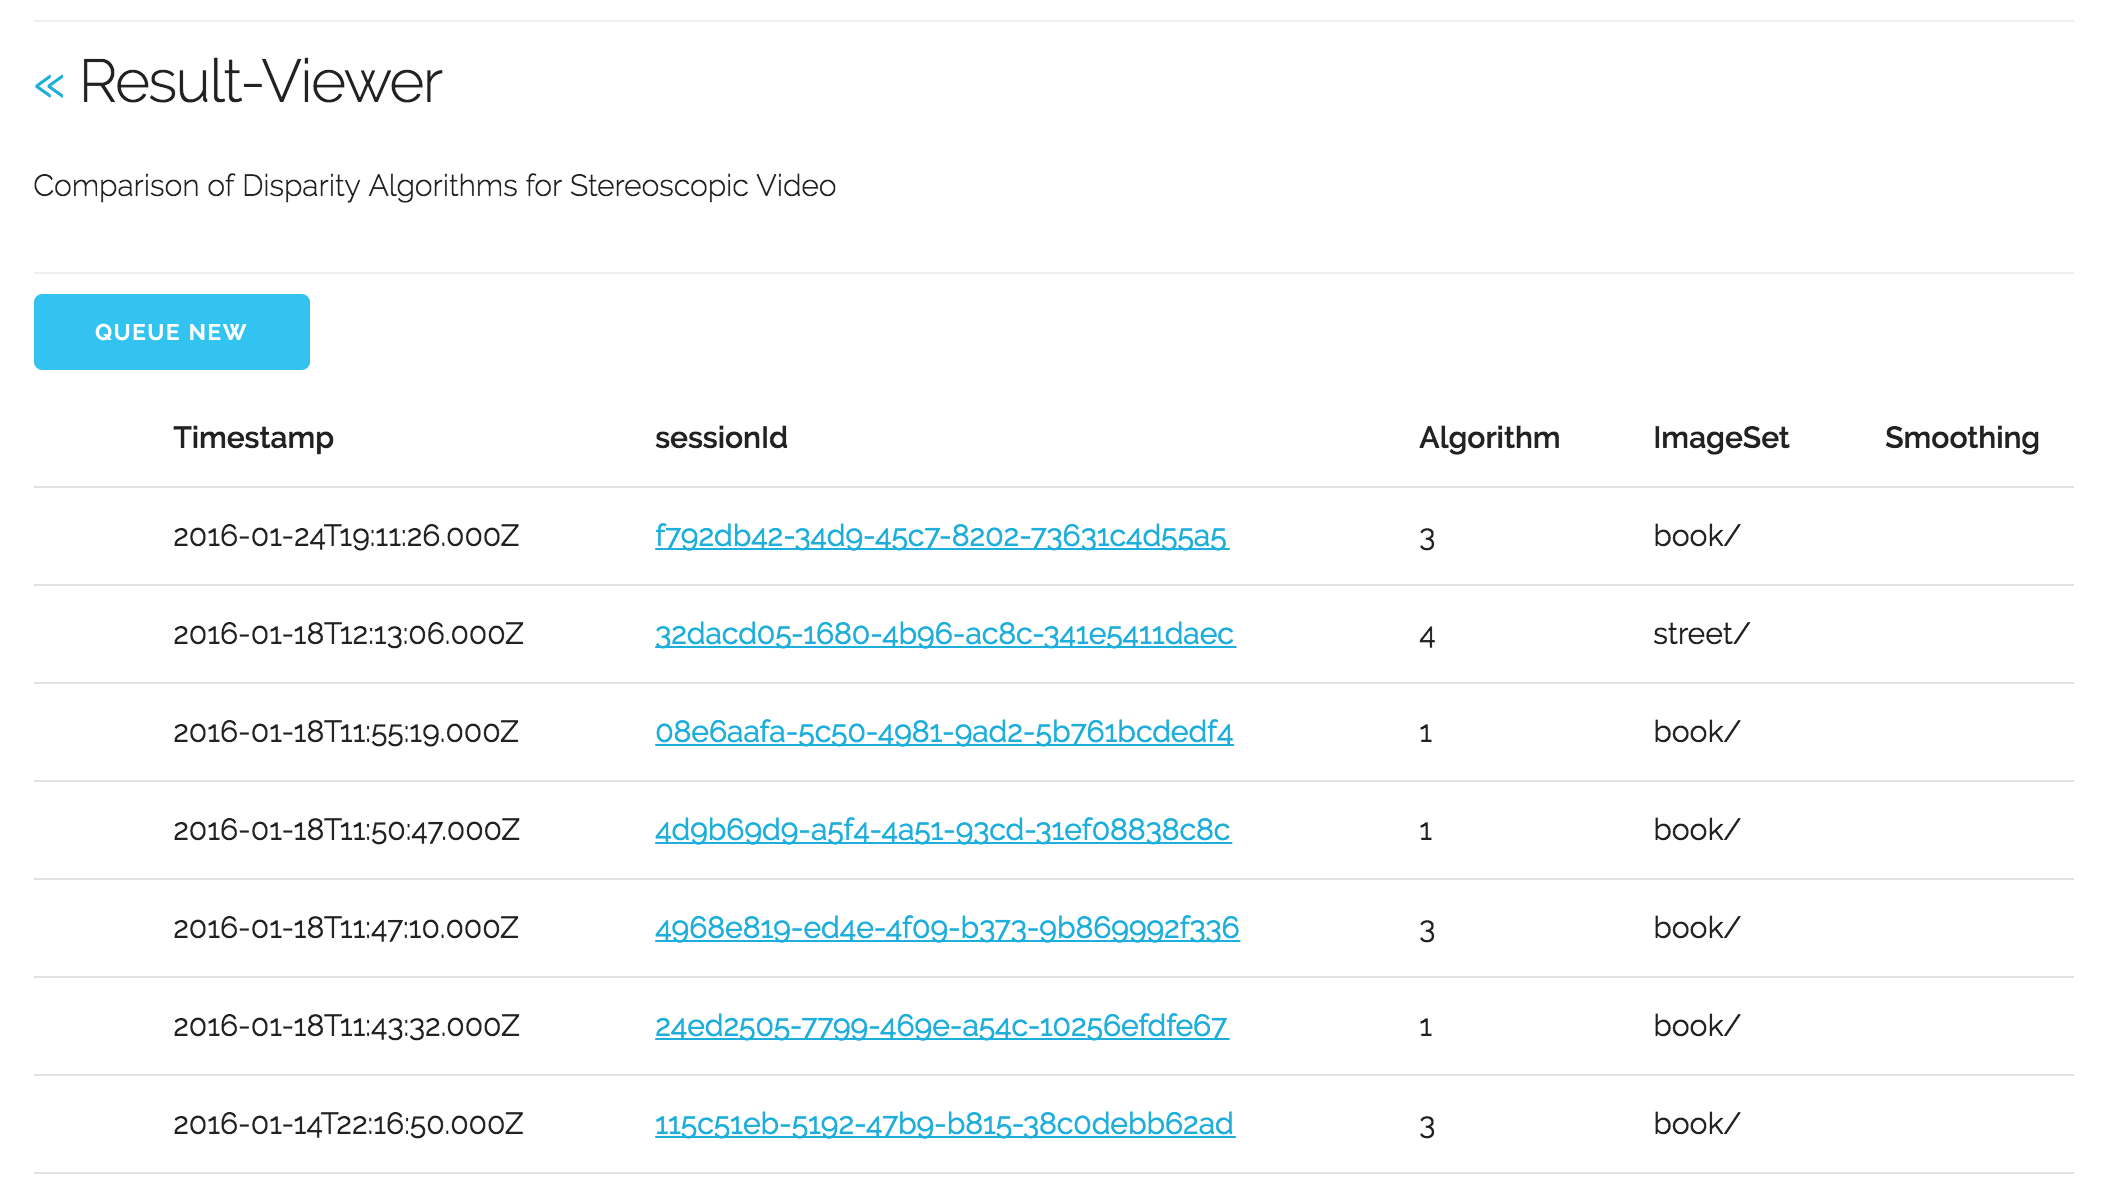
\includegraphics[angle=90,width=0.7\textwidth]{src/images/result-viewer-overview.png}
  \caption{Overview page of web result viewer.}
  \label{fig:web-overview}
\end{figure}

\begin{figure}[p!]
  \centering
  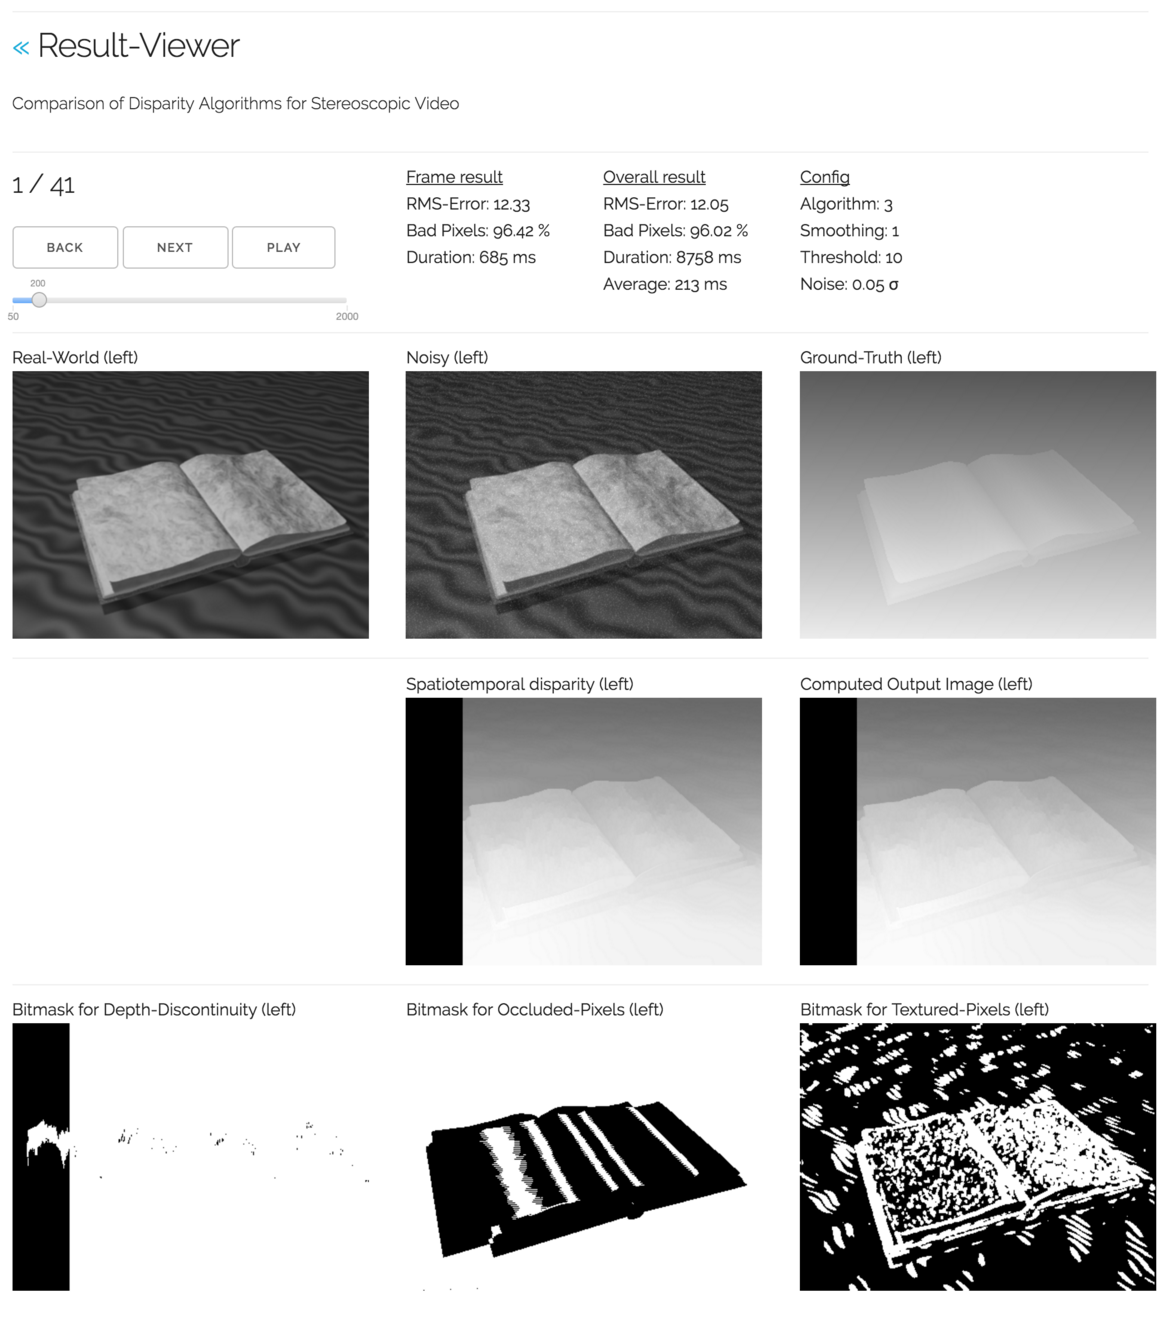
\includegraphics[angle=90,width=1.0\textwidth]{src/images/result-viewer-detail.png}
  \caption{Detail of one result in the web result viewer.}
  \label{fig:web-detail}
\end{figure}

%todo finish web result viewer section
\begin{itemize}
  \item Insert screenshot (one or two from web result viewer)
  \item Describe basic features
  \item Describe what could be done with the evaluation web suite in near future
  \item But for thesis evaluation a csv exporter was used.
\end{itemize}

\section{Discussion}

The following modules were actually implemented:

\begin{itemize}
  \item Reader for the PFM file format.
  \item Python scripts for upcoming evaluation.
  \item Shell scripts for getting the docker containers and thus the work distributed among different instances\footnote{With instances virtual machines from DigitalOcean are meant.}.
  \item Evaluation processor for
\end{itemize}
